\documentclass[8pt]{beamer}
\usetheme[secheader]{pecostalk}
\graphicspath{{figs/}}
%\usepackage{comment}
\newcommand{\paramred}[1]{{\color{red} #1}}
\newcommand{\measblue}[1]{{\color{blue} #1}}
\newcommand{\bgamma}{\bar{\gamma}}
\newcommand{\GRINS}{\texttt{GRINS}}
\newcommand{\libMesh}{\texttt{libMesh}}
\definecolor{darkgreen}{rgb}{0,0.4,0}

\setbeamerfont{normal text}{size=\small}


\title[Model Inadequacy in Supercapacitors]{
DiaMond\\
{\small Model Inadequacy in Models of Supercapacitors}
}
%\subtitle{}

\author[Moser et al]{
Robert Moser,\\ 
Danial Faghihi,
Todd Oliver,
Damien Lebrun-Grandie
$~$\\
{\small
Institute for Computational Engineering and Sciences (ICES)\\
$\quad~$The University of Texas at Austin
}
}

\date[DiaMond October 2016]{
{\it DiaMond XXXXX,
October XX, 2016
}
}

\begin{document}


%===============================================================================
% Slide 1
%===============================================================================
\begin{frame}
\frametitle{Models of Supercapacitors}
\vfill

%\vspace{0.05in}
\begin{itemize}

\item Overpotential in electrode: $\eta = \phi_{solid}-\phi_{liquid}-U_{eq}$\\
\item $\gamma$ = conductivity ratio of solid and liquid \\
\item $\xi, \tau$ = normalized space and time \\
\item $I(\tau)$ = applied current

\end{itemize}
\vspace{-0.1in}
\begin{columns}
\begin{column}{.55\textwidth}
%-----------------------------
\begin{block}{High Fidelity model}
\vspace{-0.05in}
\begin{equation*}\label{eq:HF}
\frac{\partial\eta_{HF}}{\partial\tau} = \frac{\partial^2\eta_{HF}}{\partial\xi^2}
\end{equation*}
\vspace{-0.1in}
\begin{small}
\begin{equation*}
\left\{\begin{matrix}
\frac{\partial\eta_{HF}}{\partial\xi}|_{\xi=0} & = & -\frac{\gamma}{1+\gamma}I(\tau)\\
\frac{\partial\eta_{HF}}{\partial\xi}|_{\xi=1} & = & \frac{1}{1+\gamma}I(\tau) \nonumber\\
\eta_{HF}|_{\tau=0} 					       & =  & \eta_0(\xi)
\end{matrix}\right.
\end{equation*}
\end{small}
\vspace{-0.05in}
\end{block}
%-----------------------------
\vspace{-0.08in}
\begin{block}{Low Fidelity model}
%\begin{footnotesize}
 \vspace{-0.15in}
\begin{eqnarray*}\label{eq:LF}
\eta_{LF}(\xi,\tau) = \frac{1}{2}I\xi^2- I \frac{\gamma}{1+\gamma}\xi + {\eta}^{avg}(\tau)
			 - I\frac{2\gamma-1}{6(1+\gamma)}
	\vspace{-0.3in}		 
\end{eqnarray*}
%\vspace{-0.1in}
where $\frac{\partial{\eta}^{avg}}{\partial\tau} = I$
%\vspace{-0.1in}
%\end{footnotesize}
\end{block}
%-----------------------------
\end{column}
%====================
\begin{column}{.4\textwidth}
\begin{center}
\vspace{-0.75in}
\begin{figure}[h]
    \centering
    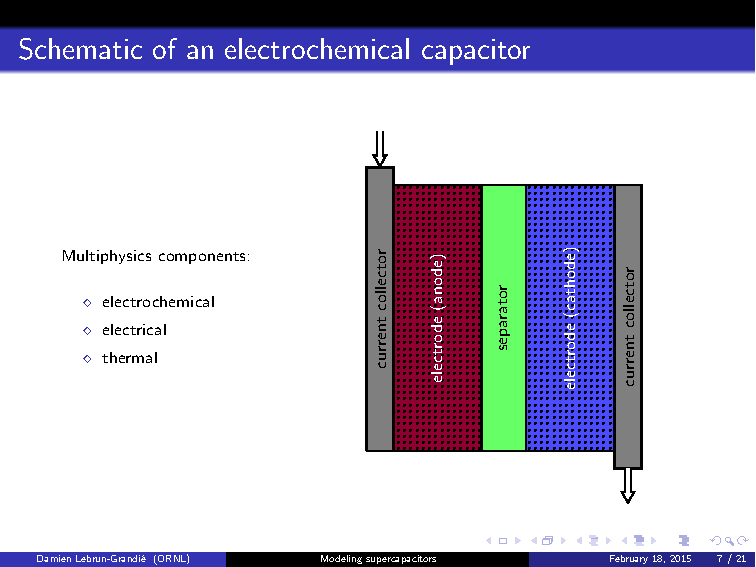
\includegraphics[trim = 2.4in 0.4in 0.7in 0.9in, clip, width=.5\textwidth]{figs_report/supercap_schematic.pdf}
    \\    \vspace{0.02in} 
    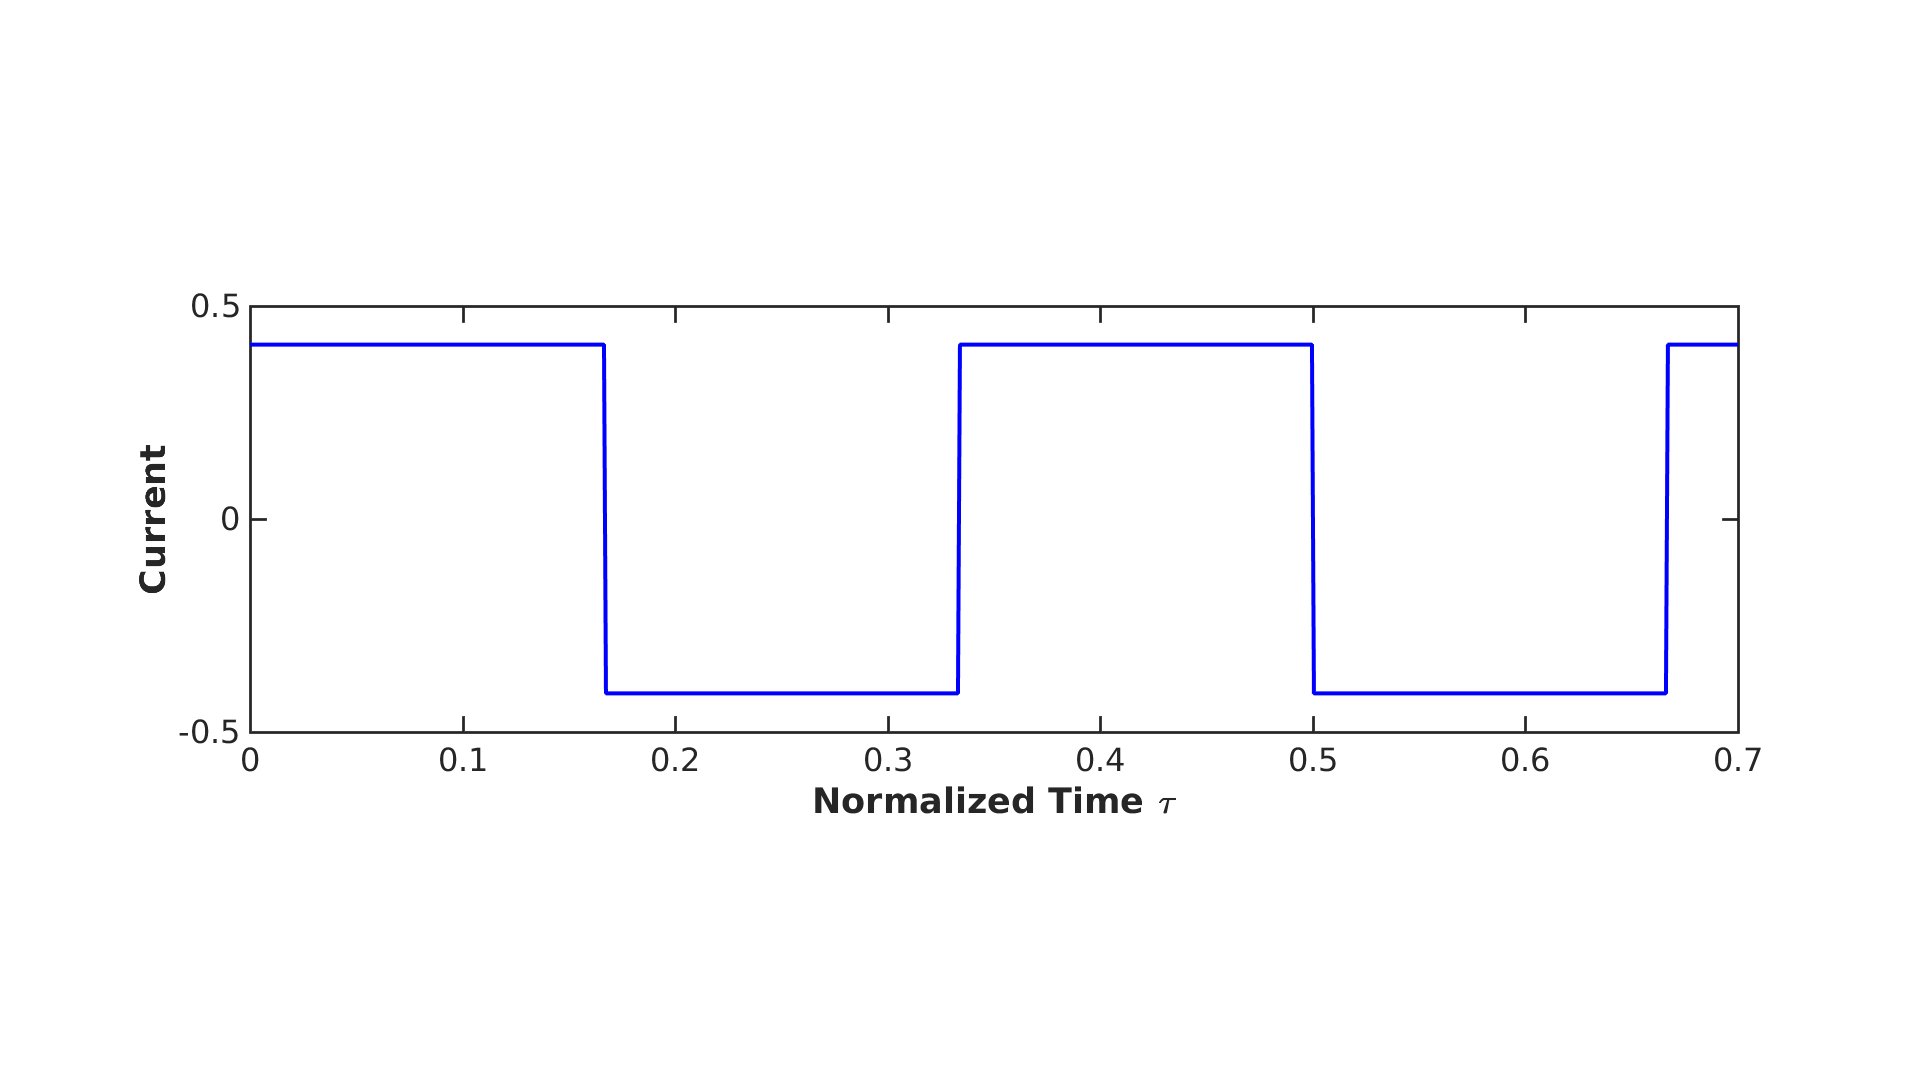
\includegraphics[trim = 1.3in 2.5in 1.6in 2.8in, clip, width=0.95\textwidth]{figs_report/I.png}
    \\
    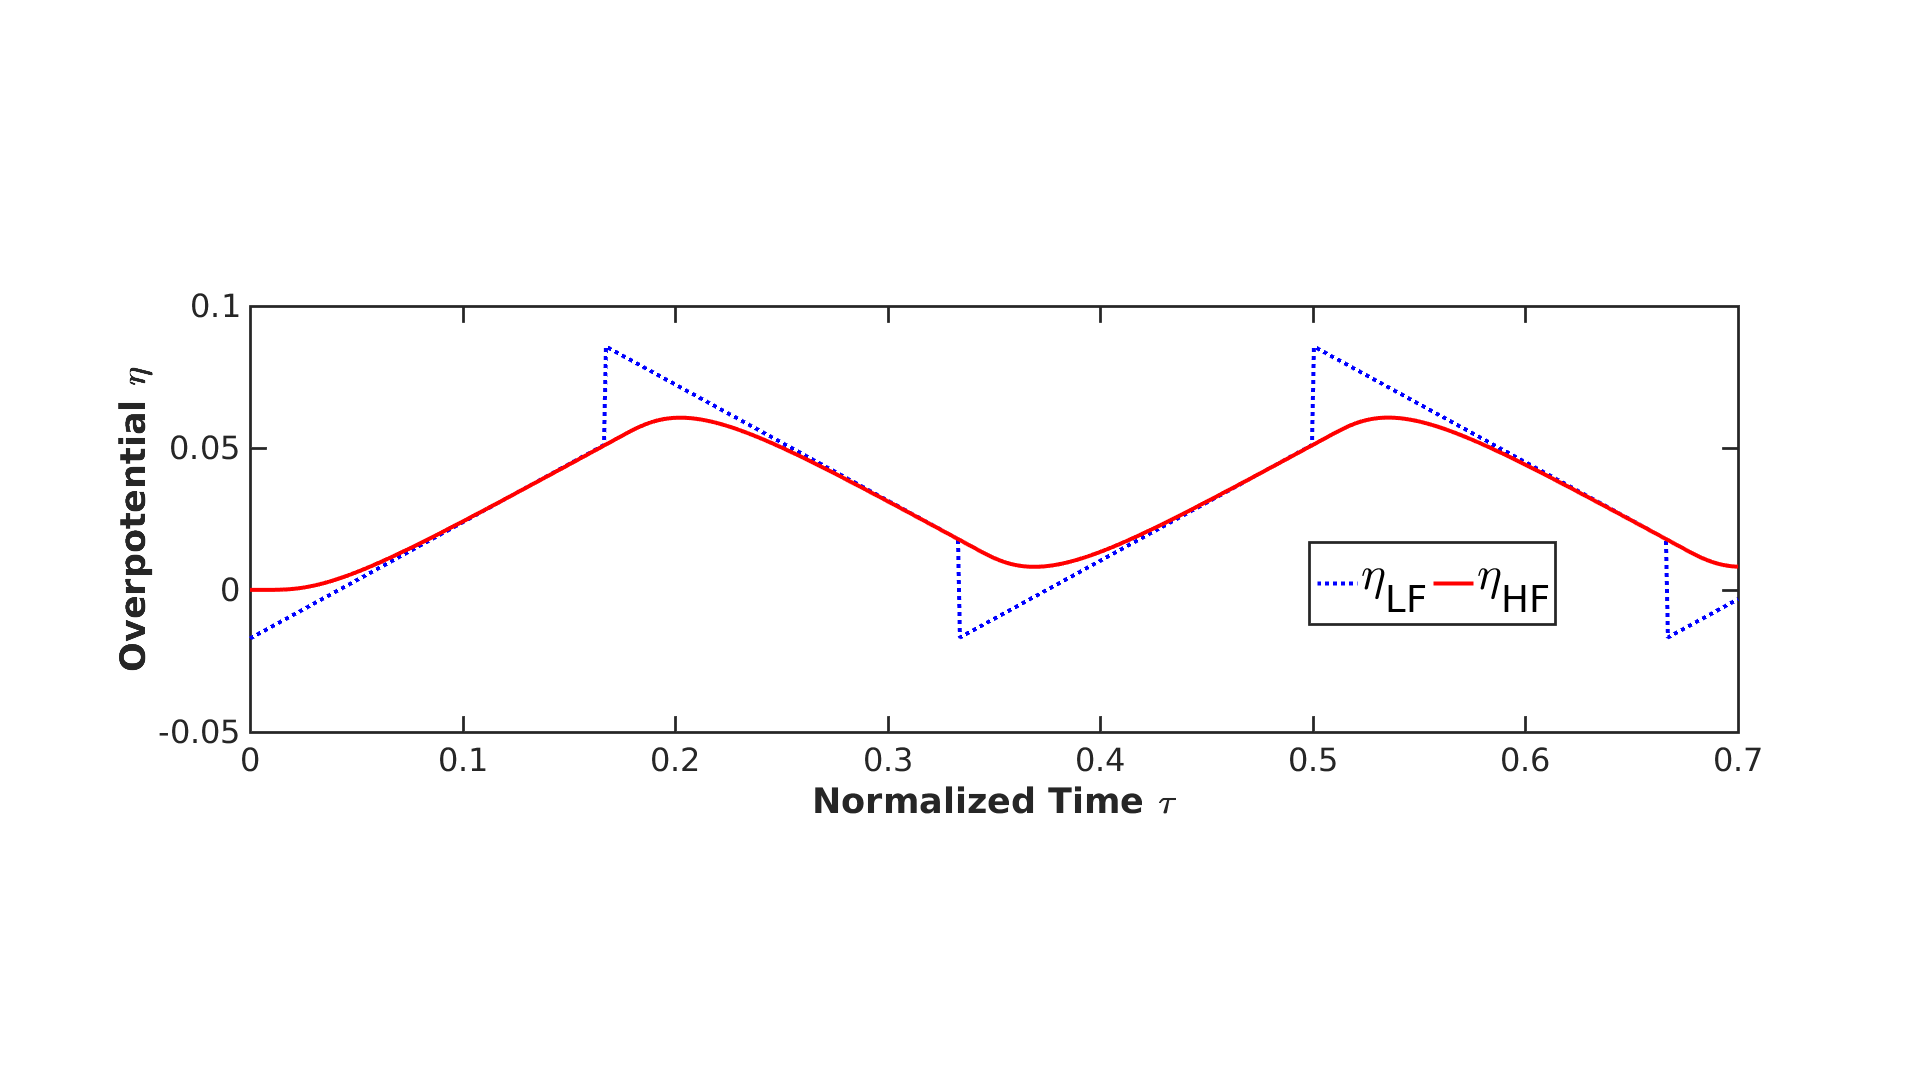
\includegraphics[trim = 1.3in 2.5in 1.6in 2.8in, clip, width=0.95\textwidth]{figs_report/etaLF_HF.png}   
\end{figure}
\end{center}
\end{column}
\end{columns}
%====================

\begin{columns}
\begin{column}{.65\textwidth}
\begin{alertblock}{Quantity of Interest}
 Potential drop across the system
 
 $V^{cell}(\tau) = \phi_{collector}^L - \phi_{collector}^R
= \frac{1+2\gamma}{1+\gamma}\eta|_{\xi=1} - \frac{\gamma}{1+\gamma}\eta|_{\xi=0} - \frac{\gamma}{(1+\gamma)^2}I
 $
\end{alertblock} 
\end{column}
%====================
\begin{column}{.3\textwidth} 
    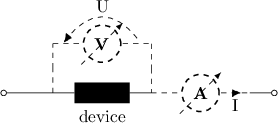
\includegraphics[trim = 0in 0in 0.in 0.2in, clip, width=0.95\textwidth]{figs_report/device.png}
\end{column}
\end{columns}



\vfill
\end{frame}

%===============================================================================
% Slide 2
%===============================================================================
\begin{frame}
\frametitle{Model Inadequacy}
\vfill

\vspace{0.1in}
\textbf{Features of Models}
\begin{itemize}
\item The high fidelity model accounts for the time history of the current. This feature is hidden in the low fidelity model. 
\item Solution of low fidelity model converge to high fidelity over time i.e. modeling error is larger for higher frequency current. 
\item Given what we know about high fidelity model $\eta_{HF}$, one can formulate inadequacy representation. 
\end{itemize}

\begin{center}
Error in QoI: \qquad
$\epsilon = V^{cell}_{HF} - V^{cell}_{LF}$
\end{center}

\vspace{0.in}
\begin{columns}
\begin{column}{.48\textwidth}
%-----------------------------
\vspace{-0.05in}
\begin{alertblock}{Inadequacy representation}

Stochastic ODE:
\begin{equation*}
\frac{\partial\epsilon}{\partial\tau} = -\lambda\epsilon + \alpha \frac{\partial I}{\partial\tau}
\end{equation*}

where $\lambda$ is a stochastic process with following time evolution:
\begin{equation*}
\frac{\partial\lambda}{\partial\tau} = -c(\lambda - \lambda_{mean}) + \beta \frac{\partial W}{\partial\tau}
\end{equation*}

where $W(t)$ is a Wiener process and $(\alpha, \beta, c, \lambda_{mean})$ are parameters of inadequacy representation. 
\end{alertblock}

\end{column}
%====================
\begin{column}{.48\textwidth}
\begin{center}
\vspace{-4mm}
\begin{figure}[h]
    \centering
    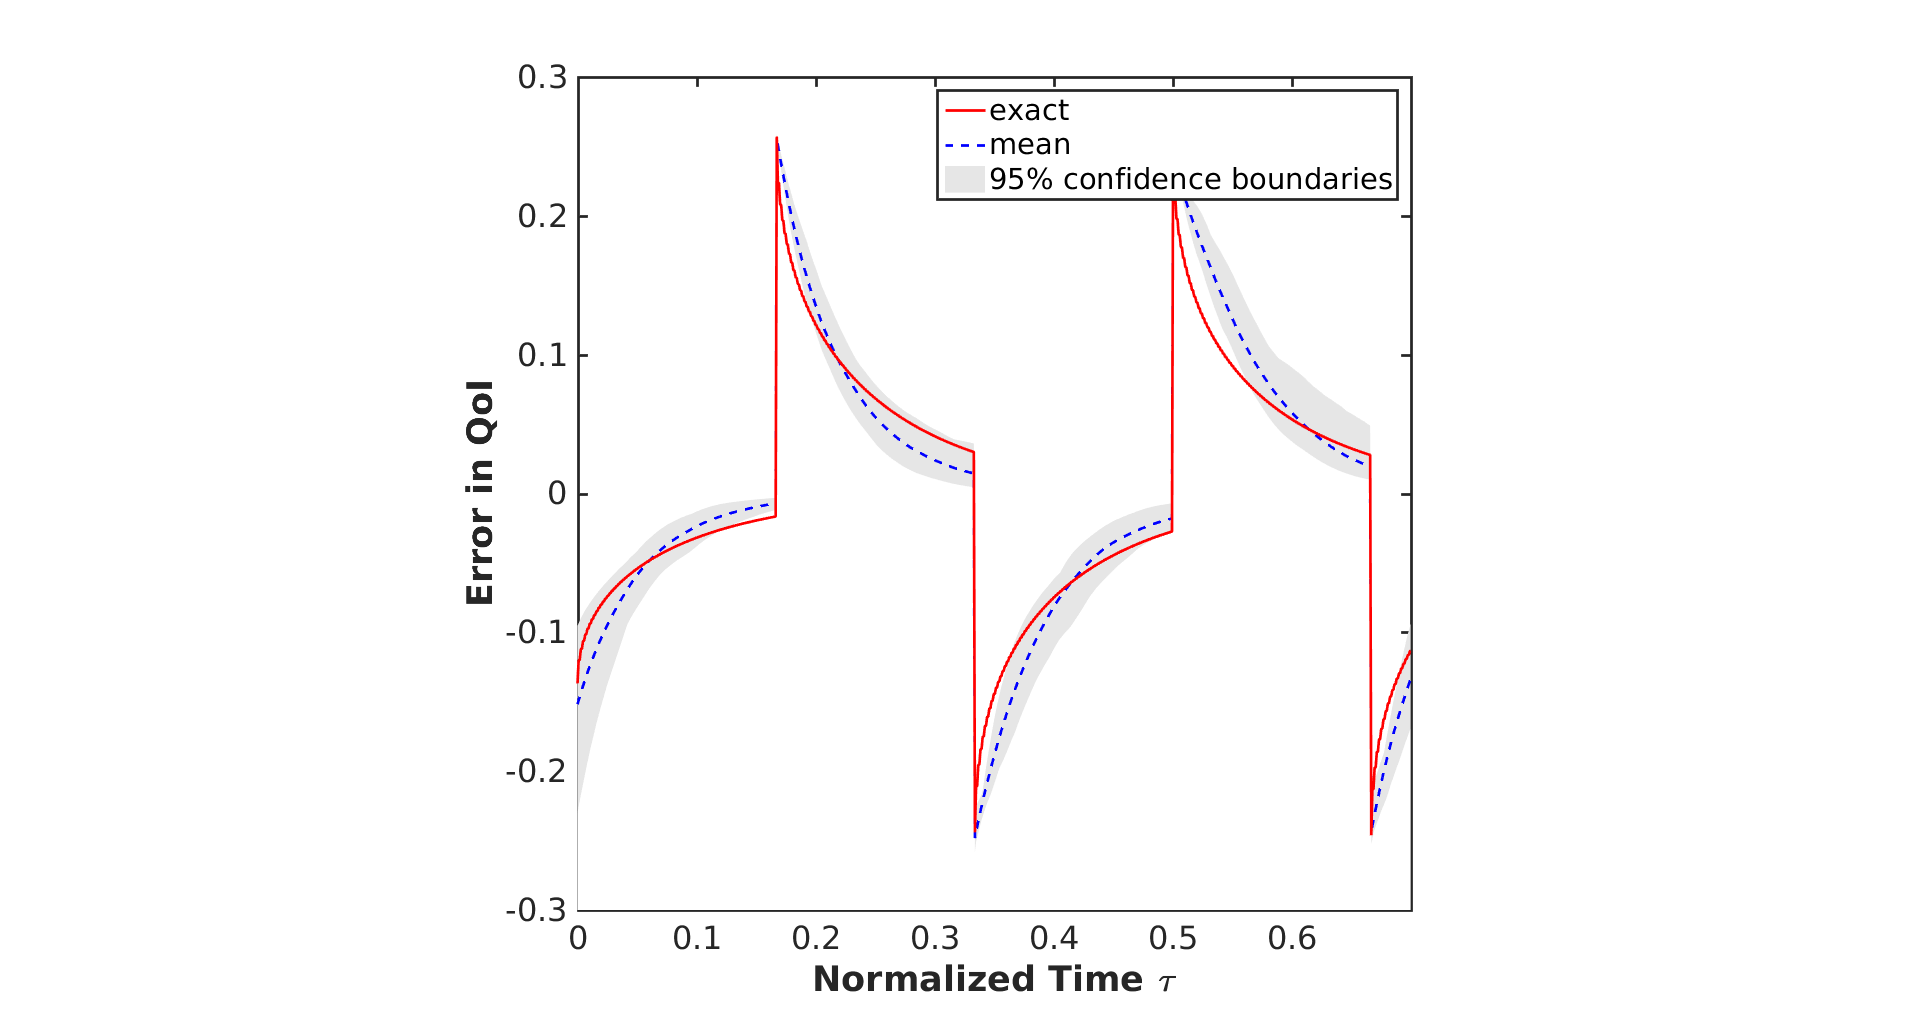
\includegraphics[trim = 4in 0.1in 4in 0.1in, clip, width=1\textwidth]{figs_report/error_bound.png} 
\end{figure}
\end{center}
\end{column}
\end{columns}
\vspace{2mm}

\vfill
\end{frame}

\end{document}

